\documentclass{beamer}
\usepackage[utf8]{inputenc}
\usepackage{graphicx, epsfig}
\usepackage{amsmath,mathrsfs,amsfonts,amssymb}
\usepackage{floatflt}
\usepackage{epic,ecltree}
\usepackage{mathtext}
\usepackage{fancybox}
\usepackage{fancyhdr}
\usepackage{multirow}
\usepackage{enumerate}
\usepackage{epstopdf}
\usepackage{multicol}
\usepackage{algorithm}
\usepackage[noend]{algorithmic}
\usepackage{tikz}
\usepackage{blindtext}
\usetheme{default}%{Singapore}%{Warsaw}%{Warsaw}%{Darmstadt}
\usecolortheme{default}

\setbeamerfont{title}{size=\Huge}
\setbeamertemplate{footline}[page number]{}

\setbeamertemplate{section in toc}[sections numbered]


\makeatletter
\newcommand\HUGE{\@setfontsize\Huge{35}{40}}
\makeatother    

\setbeamerfont{title}{size=\HUGE}
\beamertemplatenavigationsymbolsempty

% latin bold lower
\newcommand{\ba}{\mathbf{a}} 
\newcommand{\bc}{\mathbf{c}} 
\newcommand{\be}{\mathbf{e}} 
\newcommand{\bh}{\mathbf{h}} 
\newcommand{\bp}{\mathbf{p}} 
\newcommand{\bt}{\mathbf{t}} 
\newcommand{\bs}{\mathbf{s}} 
\newcommand{\bu}{\mathbf{u}} 
\newcommand{\bv}{\mathbf{v}} 
\newcommand{\bw}{\mathbf{w}} 
\newcommand{\bx}{\mathbf{x}} 
\newcommand{\by}{\mathbf{y}} 
\newcommand{\bz}{\mathbf{z}} 

% latin bold upper
\newcommand{\bA}{\mathbf{A}} 
\newcommand{\bB}{\mathbf{B}} 
\newcommand{\bC}{\mathbf{C}} 
\newcommand{\bI}{\mathbf{I}} 
\newcommand{\bJ}{\mathbf{J}} 
\newcommand{\bL}{\mathbf{L}} 
\newcommand{\bM}{\mathbf{M}} 
\newcommand{\bQ}{\mathbf{Q}} 
\newcommand{\bT}{\mathbf{T}} 
\newcommand{\bU}{\mathbf{U}} 
\newcommand{\bV}{\mathbf{V}} 
\newcommand{\bW}{\mathbf{W}} 
\newcommand{\bX}{\mathbf{X}} 
\newcommand{\bY}{\mathbf{Y}} 
\newcommand{\bZ}{\mathbf{Z}} 

% latin cal upper
\newcommand{\cG}{\mathcal{G}} 
\newcommand{\cL}{\mathcal{L}} 
\newcommand{\cN}{\mathcal{N}} 
\newcommand{\cS}{\mathcal{S}} 
\newcommand{\cT}{\mathcal{T}} 
\newcommand{\cW}{\mathcal{W}} 
\newcommand{\cX}{\mathcal{X}} 
\newcommand{\cZ}{\mathcal{Z}} 

% latin bb upper
\newcommand{\bbE}{\mathbb{E}} 
\newcommand{\bbI}{\mathbb{I}} 
\newcommand{\bbP}{\mathbb{P}} 
\newcommand{\bbR}{\mathbb{R}} 

% greek bold lower
\newcommand{\bepsilon}{\boldsymbol{\epsilon}} 
\newcommand{\btheta}{\boldsymbol{\theta}} 
\newcommand{\blambda}{\boldsymbol{\lambda}} 
\newcommand{\bpi}{\boldsymbol{\pi}} 
\newcommand{\bmu}{\boldsymbol{\mu}} 
\newcommand{\bsigma}{\boldsymbol{\sigma}} 
\newcommand{\bphi}{\boldsymbol{\phi}} 

% greek bold upper
\newcommand{\bSigma}{\boldsymbol{\Sigma}} 

\DeclareMathOperator*{\argmin}{arg\,min}
\DeclareMathOperator*{\argmax}{arg\,max}

\newcommand{\createdgmtitle}[1]{\title[\hbox to 56mm{Deep Learning Audio \hfill\insertframenumber\,/\,\inserttotalframenumber}]
	{\vspace{1cm} \\ Deep Learning Audio \\ {\Huge Lecture #1}}
	\author{Pavel Severilov}
	\institute{
	Moscow Institute of Physics and Technology
	} 
	\date{2022}
}

\newcommand\myfootnote[1]{%
  \tikz[remember picture,overlay]
  \draw (current page.south west) +(1in + \oddsidemargin,0.5em)
  node[anchor=south west,inner sep=0pt]{\parbox{\textwidth}{%
      \rlap{\rule{10em}{0.4pt}}\raggedright\scriptsize \textit{#1}}};}

\newcommand\myfootnotewithlink[2]{%
  \tikz[remember picture,overlay]
  \draw (current page.south west) +(1in + \oddsidemargin,0.5em)
  node[anchor=south west,inner sep=0pt]{\parbox{\textwidth}{%
      \rlap{\rule{10em}{0.4pt}}\raggedright\scriptsize\href{#1}{\textit{#2}}}};}
      
\AtBeginSection[]
{
	\begin{frame}{Outline}
		\tableofcontents[currentsection,subsectionstyle=hide]
	\end{frame}
}
\AtBeginSubsection[]{
	\begin{frame}{Outline}
		\tableofcontents[currentsection,currentsubsection]
	\end{frame}
}
\createdgmtitle{3}
\usepackage{tikz}
\usetikzlibrary{arrows,shapes,positioning,shadows,trees}
%--------------------------------------------------------------------------------
\begin{document}
%--------------------------------------------------------------------------------
\begin{frame}[noframenumbering,plain]
%\thispagestyle{empty}
\titlepage
\end{frame}
%=======x
\begin{frame}{Outline}
	\tableofcontents
\end{frame}
%=======
\section{Automatic Speech Recognition (ASR)}
%=======
\begin{frame}{ASR: Task definition}
    Mapping: signal $x(t) \rightarrow$ text sequence $s$ 
    \begin{figure}
    	\centering
    	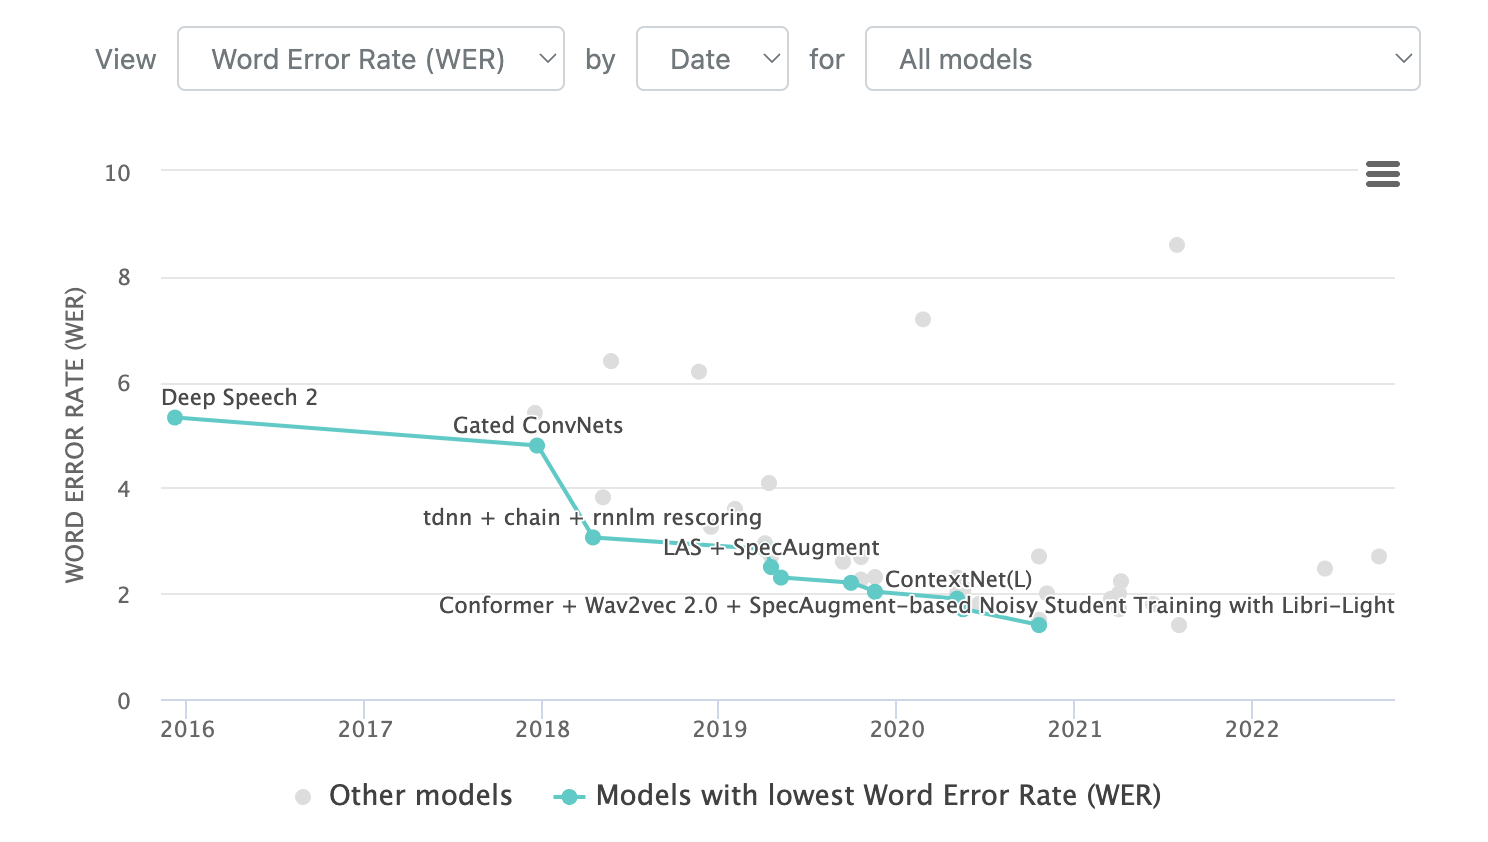
\includegraphics[width=0.99\linewidth]{figs/asr.png}
    	\caption{ASR progress for WER metric}
    \end{figure}
\end{frame}
%=======
\begin{frame}{ASR: Metrics}
    \textbf{Word Error Rate} $$WER=\frac{S+D+I}{N}=\frac{S+D+I}{S+D+C}$$
    \begin{itemize}
        \item $S$ - number of substitutions,
        \item $D$ - number of deletions,
        \item $I$ - number of insertions,
        \item $C$ - number of correct words,
        \item $N$ - number of words in the reference ($N=S+D+C$).
    \end{itemize}
    \begin{figure}
    	\centering
    	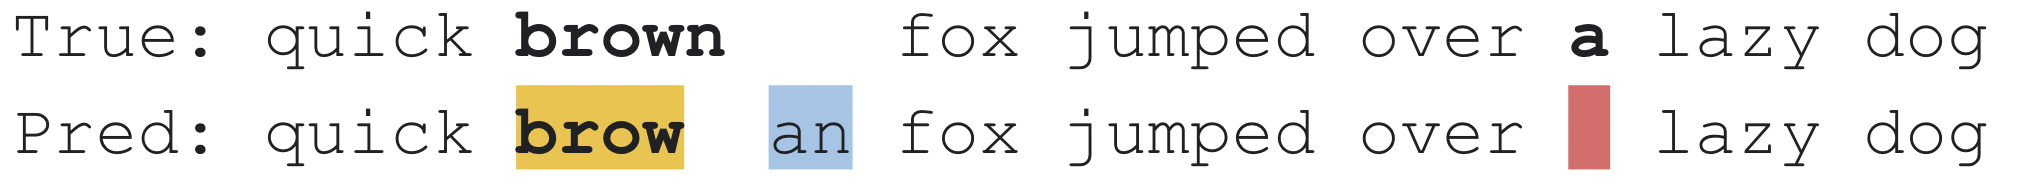
\includegraphics[width=0.99\linewidth]{figs/wer.png}
    \end{figure}

    \textbf{Character Error Rate}: same as WER, but for characters (WER is more important)
\end{frame}
%=======
\begin{frame}{ASR: Datasets: LibriSpeech}
\begin{itemize}
    \item 1,000 hours of audiobooks
    \item 10-20s audio, long sentences, complex language
    \item ’clean’ (low-WER speakers) and ’other’ (high-WER speakers) categories
    \item Human WER: test-clean: 5.83, test-other: 12.69
    \item Kaldi (2015) WER: test-clean:  8.01, test-other: 22.49
    \item  Deep Speech 2 (2015) WER: test-clean:  5.15, test-other: 12.73


\end{itemize}
    \begin{figure}
    	\centering
    	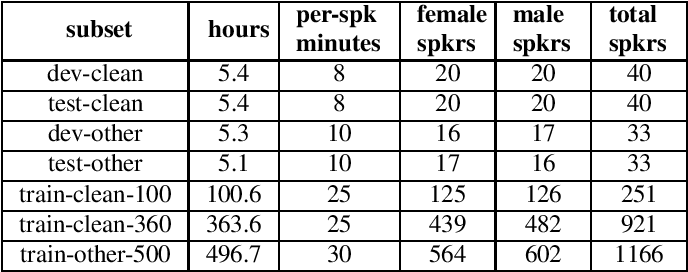
\includegraphics[width=0.8\linewidth]{figs/librispeech.png}
    \end{figure}

	\myfootnotewithlink{http://kaldi-asr.org/}{Kaldi ASR by Daniel Povey}

    
\end{frame}
%=======
\begin{frame}{ASR: Datasets: Mozilla Common Voice}
\begin{itemize}
    \item Multiple languages
    \item Crowdsourced
    \item Simple language
    \item Short phrases
    \item Frequently updated and validated

\end{itemize}
    \begin{figure}
    	\centering
    	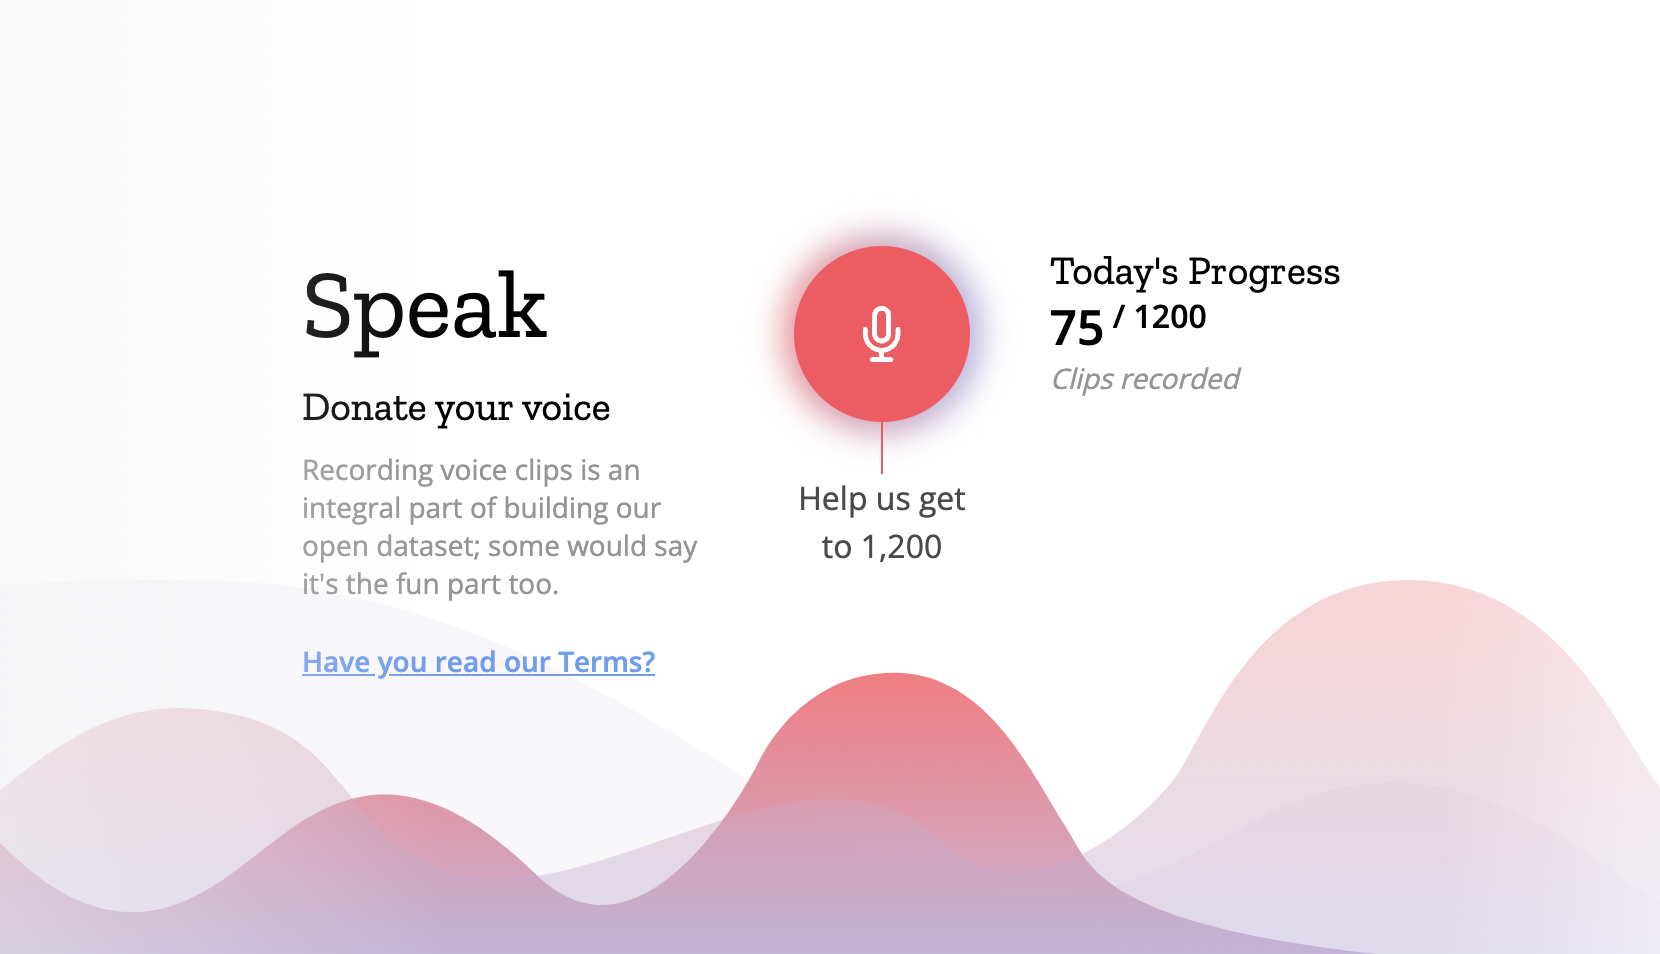
\includegraphics[width=0.8\linewidth]{figs/mozilla.png}
    \end{figure}

	\myfootnotewithlink{https://commonvoice.mozilla.org/en}{Mozilla Common Voice}

\end{frame}

%=======
\section{Connectionist Temporal Classification (CTC)}
%=======
\begin{frame}{CTC: motivation}
\begin{itemize}
    \item Variable length input
    \item Variable length output
    \item No alignment
    \item Want a differentiable loss function to compute $P(Y | X)$ and $\argmax{P(Y | X)}$

\end{itemize}

    \begin{figure}
    	\centering
    	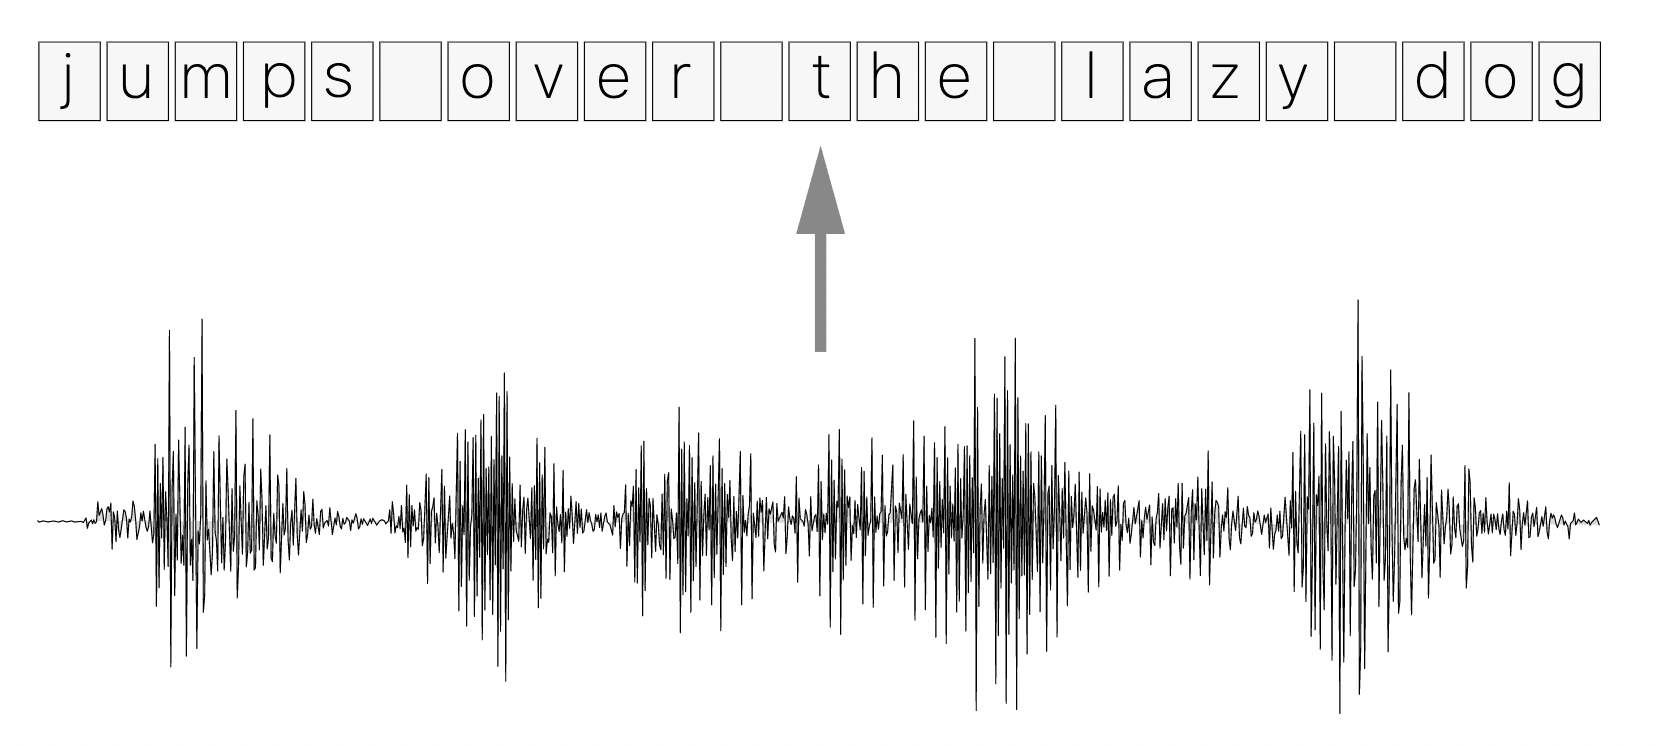
\includegraphics[width=0.8\linewidth]{figs/ctc_motivation.png}
    \end{figure}
    
    \myfootnotewithlink{https://distill.pub/2017/ctc/}{Sequence Modeling With CTC blog post}
\end{frame}

%=======
\begin{frame}{CTC: idea}
\begin{itemize}
    \item Split input into frames
    \item Classify each frame into letters classes
    \item Merge consecutive letters
    
    \begin{figure}
    	\centering
    	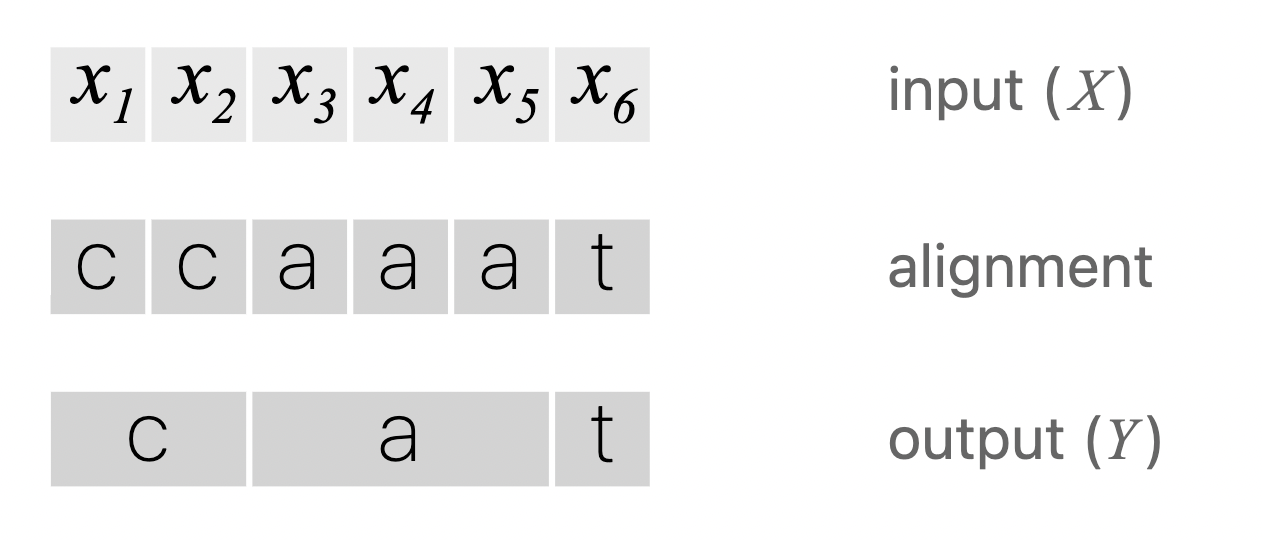
\includegraphics[width=0.8\linewidth]{figs/ctc_idea.png}
    	\caption{Example for [c, a ,t]}

    \end{figure}
\end{itemize}
\end{frame}

%=======
\begin{frame}{DeepSpeech 2}

    \begin{figure}
    	\centering
    	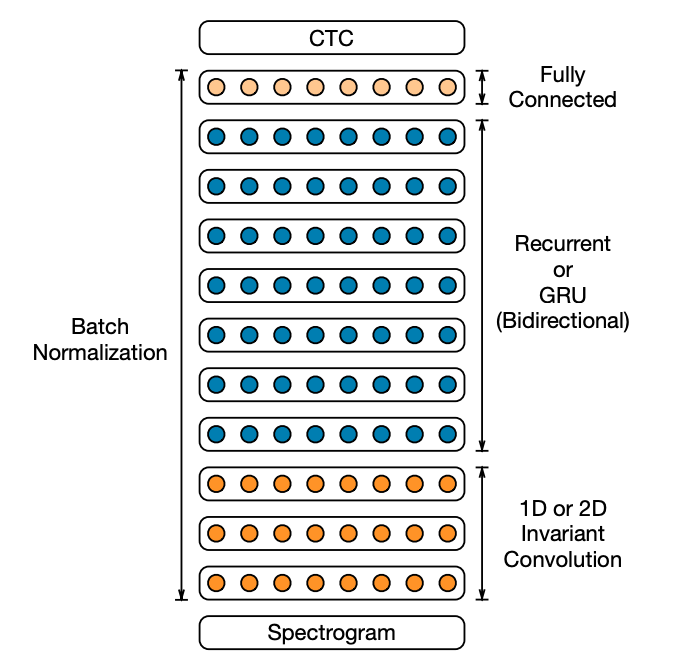
\includegraphics[width=0.6\linewidth]{figs/deepspeech.png}
    	\caption{Deep Speech 2 architecture}

    \end{figure}

	\myfootnotewithlink{https://arxiv.org/abs/1512.02595}{Amodei, Dario & Ananthanarayanan et al. (2015). Deep Speech 2: End-to-End Speech Recognition in English and Mandarin. } 
\end{frame}

%=======
\begin{frame}{CTC: problems}
Multiple consecutive letters (e.g.: hello), silence between words and letters.

\textbf{Solution}: add empty token $\epsilon$
    \begin{figure}
    	\centering
    	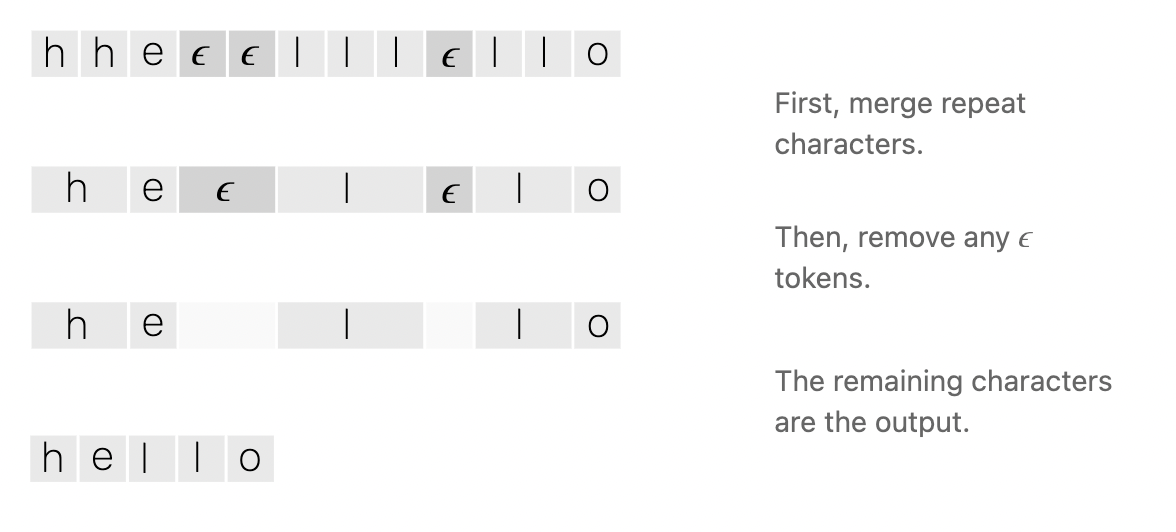
\includegraphics[width=0.9\linewidth]{figs/ctc_emptytoken.png}
    	\caption{Example for [h, e, l, l, o]}

    \end{figure}
\end{frame}

%=======
\begin{frame}{CTC: Loss function}
    \begin{figure}
    	\centering
    	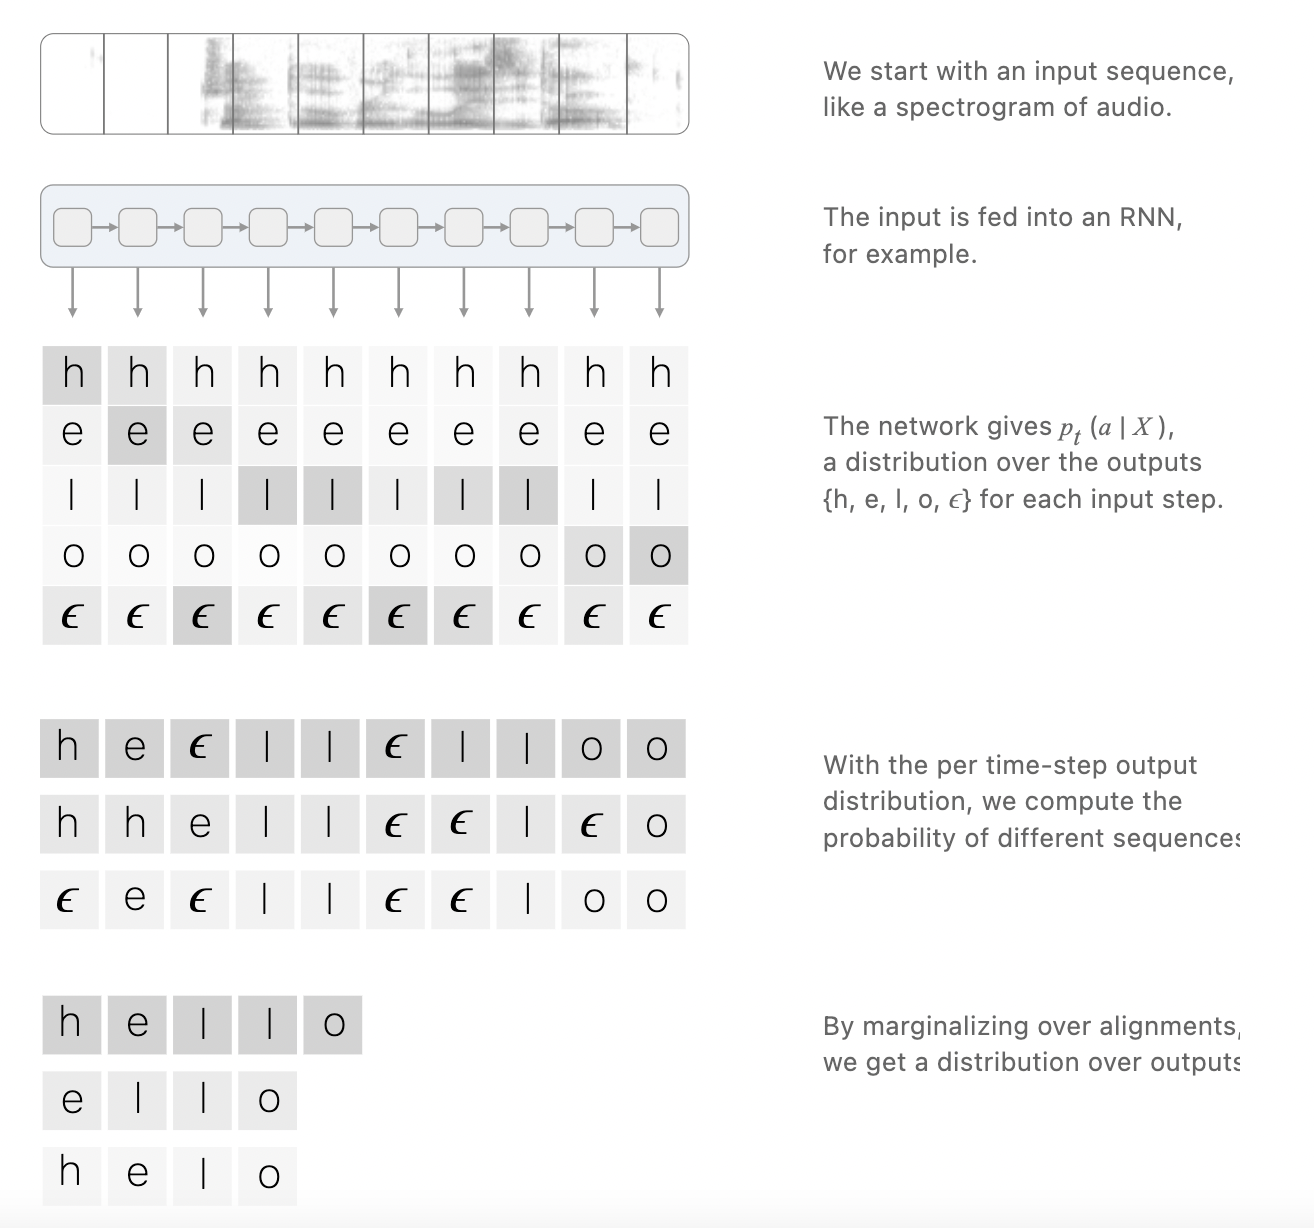
\includegraphics[width=0.7\linewidth]{figs/ctc_main.png}
    	\caption{The CTC alignments give us a natural way to go from probabilities at each time-step to the probability of an output sequence.}

    \end{figure}
\end{frame}
%=======
\begin{frame}{CTC: Loss function}
    \begin{figure}
    	\centering
    	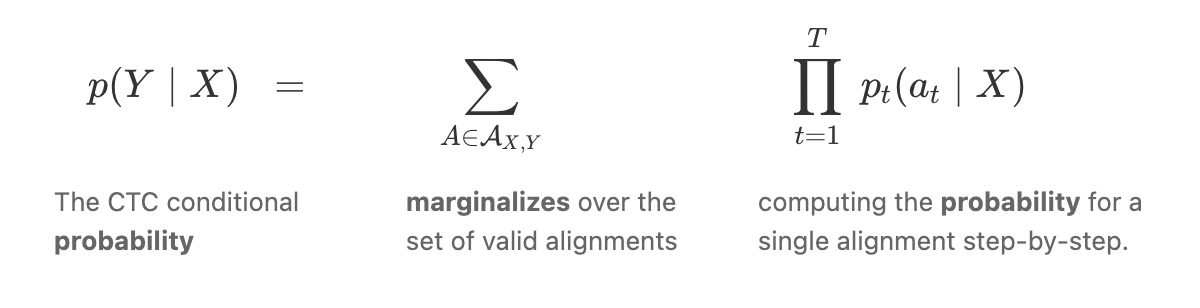
\includegraphics[width=0.99\linewidth]{figs/ctc_loss.png}
    	\caption{The CTC conditional probability}
    \end{figure}
  
      \begin{figure}
    	\centering
    	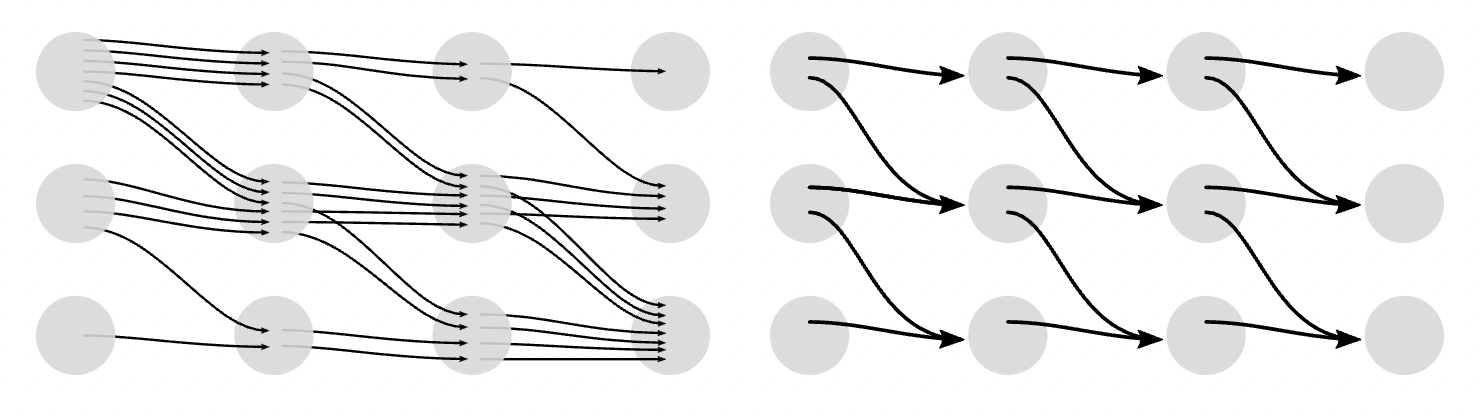
\includegraphics[width=0.99\linewidth]{figs/computation_problem_ctc.png}
    	\caption{Summing over all alignments can be very expensive. Dynamic programming merges alignments, so it’s much faster.}
    \end{figure}  

\end{frame}
%=======
\begin{frame}{CTC: Computation}
    \begin{figure}
    	\centering
    	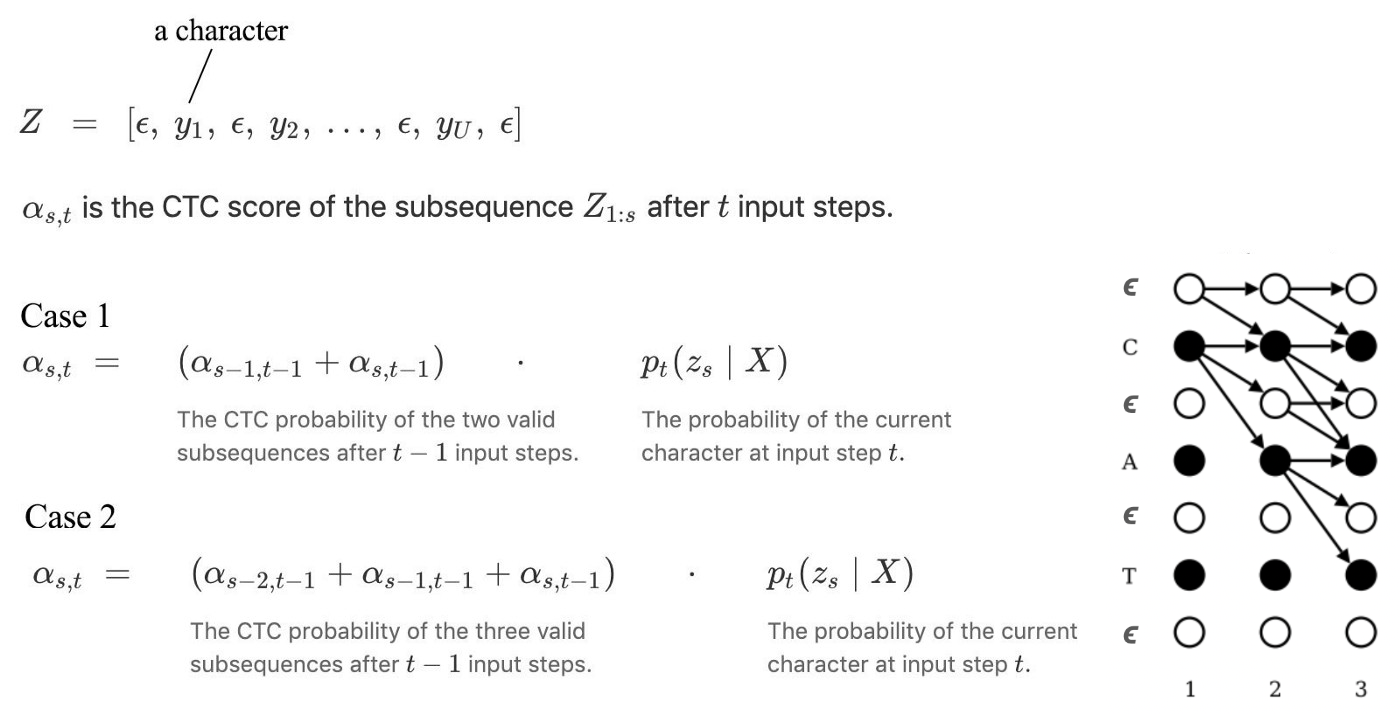
\includegraphics[width=0.99\linewidth]{figs/ctc_computation.png}
    	\caption{CTC computation with Dynamic programming}

    \end{figure}
    
\end{frame}
%=======
\begin{frame}{CTC: Properties}
\begin{itemize}
    \item Problem: Conditional Independence
    \item Example: "AAA". If predict ‘A’ as the first letter -- suffix ‘AA’ should get much more probability than ‘riple A’. If predict ‘t’ first -- the opposite.
    \begin{figure}
    	\centering
    	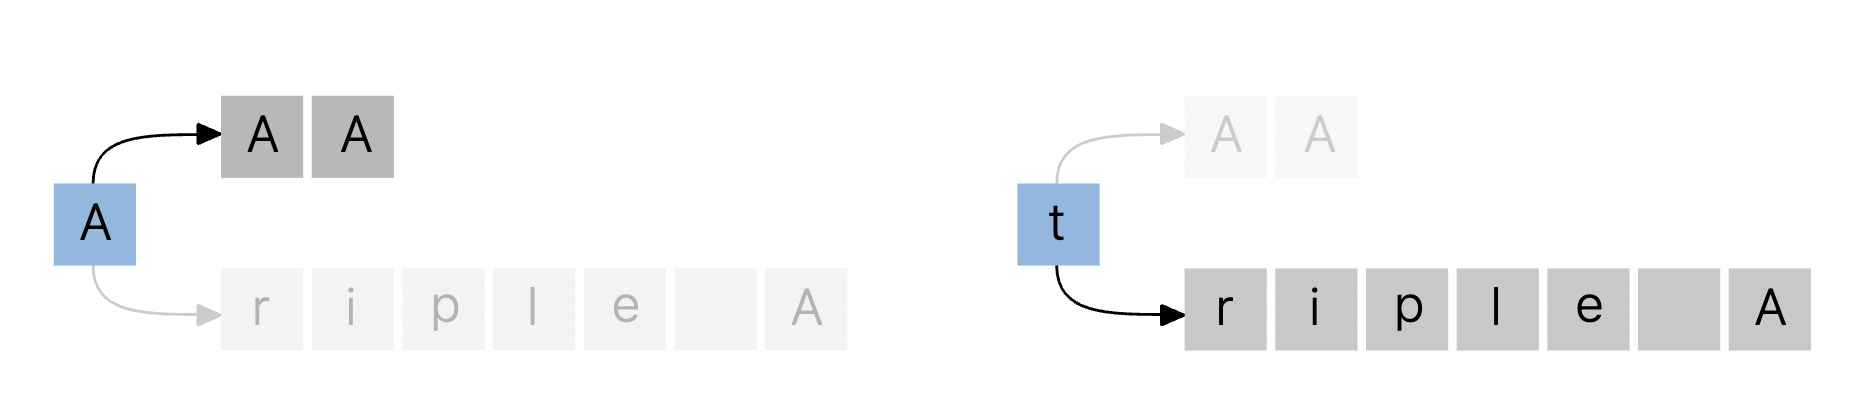
\includegraphics[width=0.9\linewidth]{figs/ctc_problem.png}
    	\caption{Valid transcription could be "AAA" and "triple A".}

    \end{figure}
    
    \item Advantage: Online -- can be performed while the speaker is talking
\end{itemize}

\end{frame}
%=======
\begin{frame}{CTC: Beam search}
    \begin{figure}
    	\centering
    	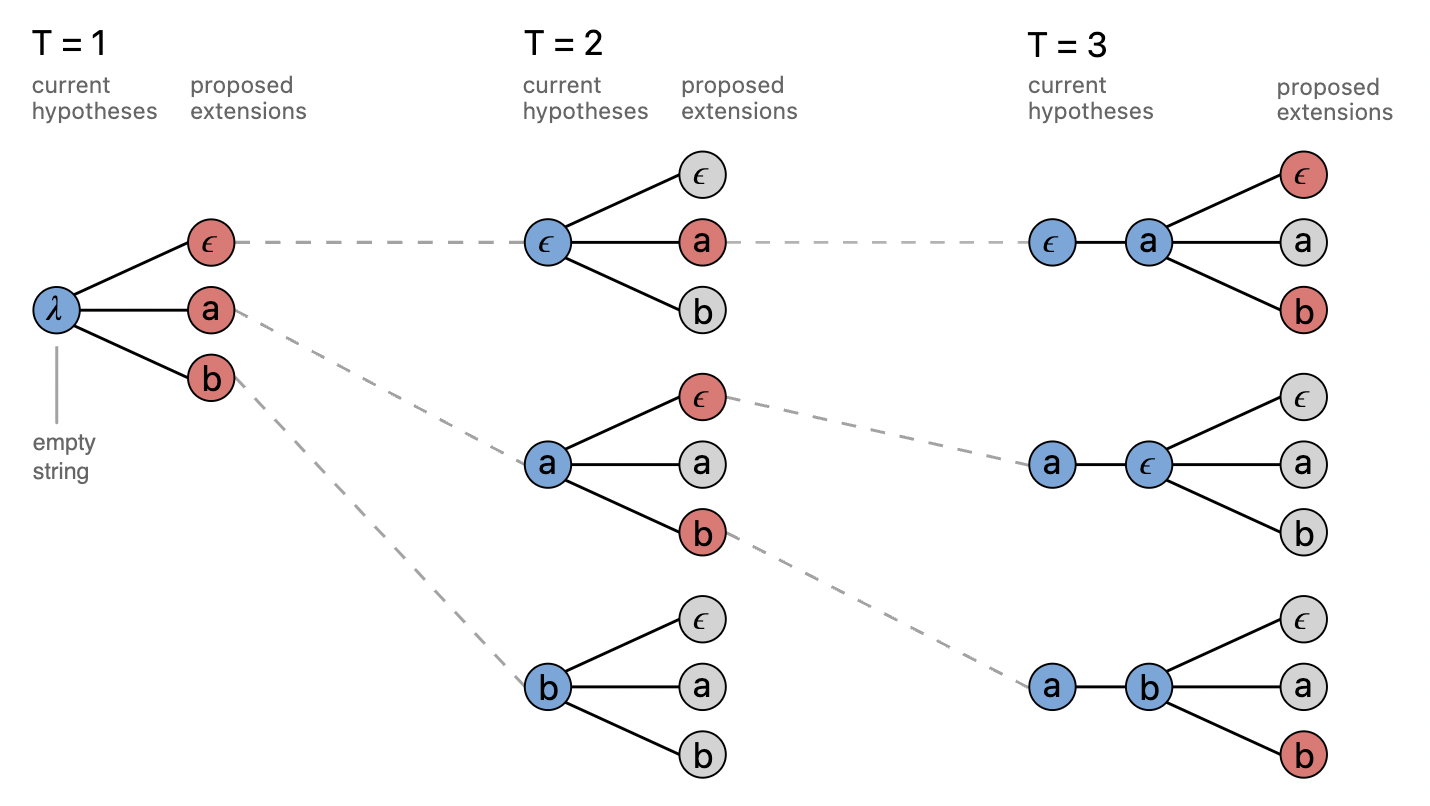
\includegraphics[width=0.9\linewidth]{figs/beam_search.png}
    	\caption{A standard beam search algorithm with an alphabet of $\{\epsilon, a, b\}$ and a beam size of 3.}

    \end{figure}
\end{frame}

%=======
\section{Listen, Attend and Spell (LAS)}
%=======
\begin{frame}{LAS: Architecture}
    \begin{figure}
    	\centering
    	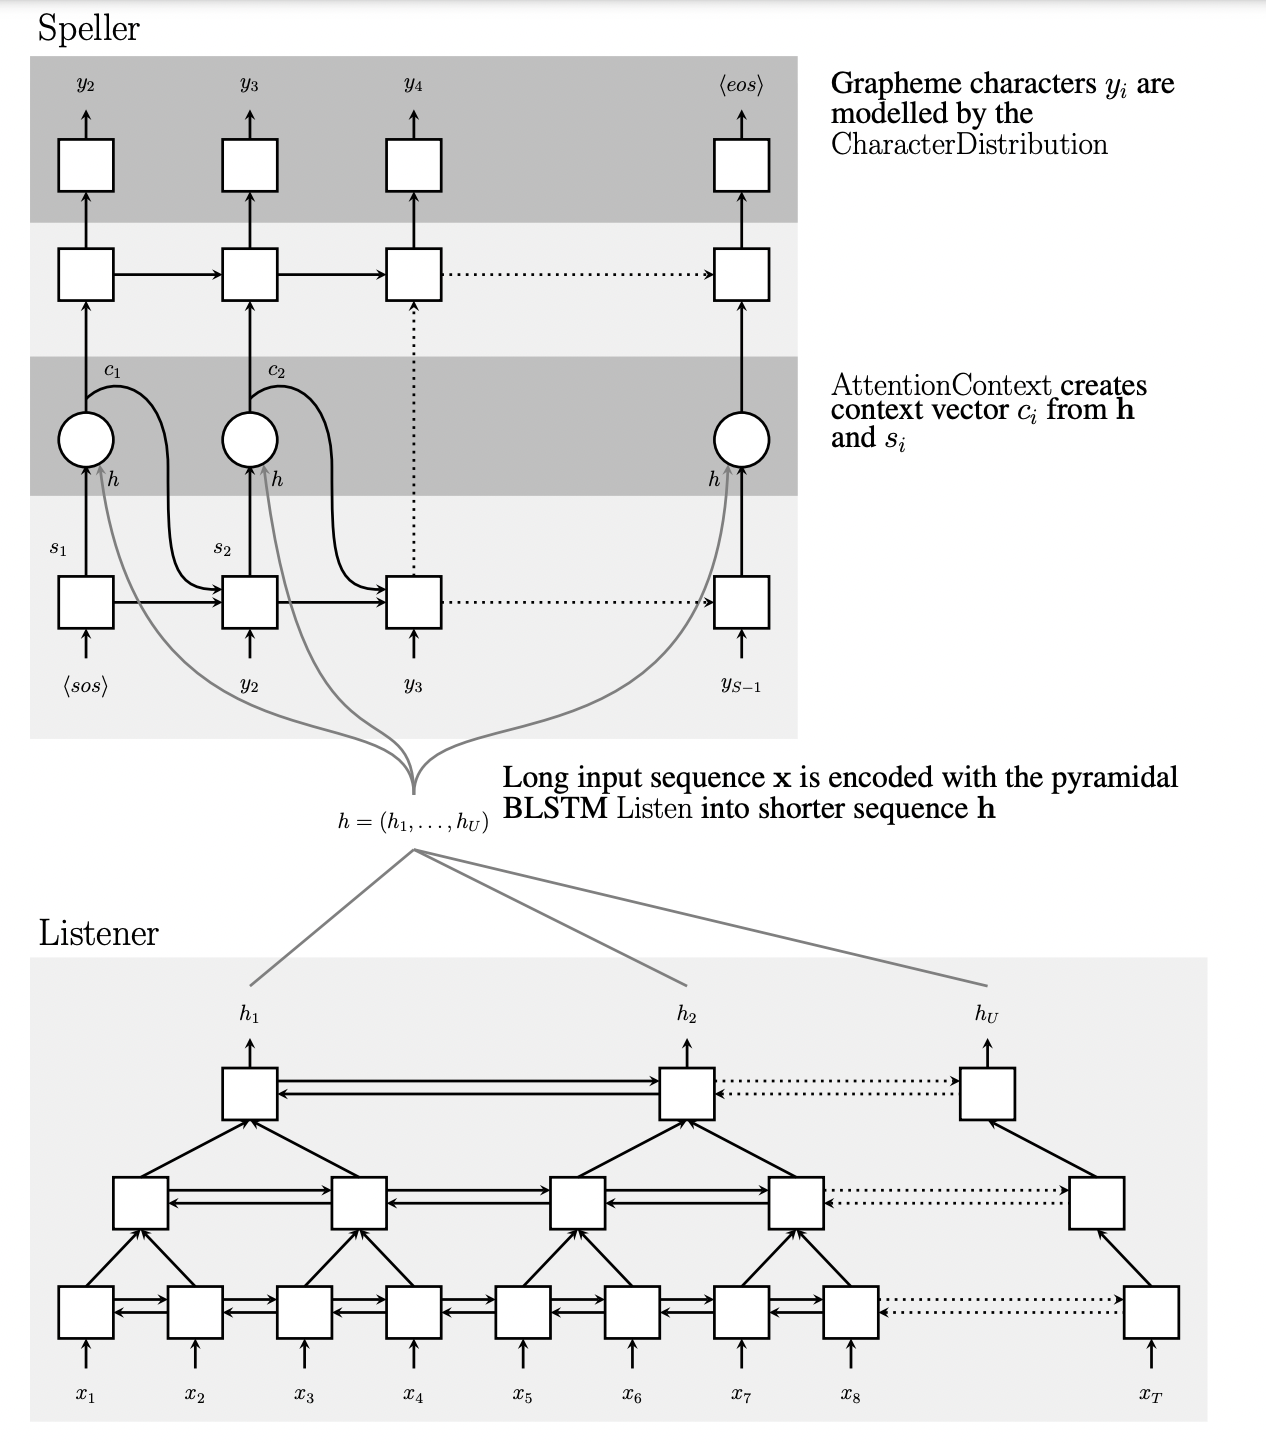
\includegraphics[width=0.55\linewidth]{figs/las.png}
    	\caption{LAS model: \textbf{listener} -- pyramidal BiLSTM encoding input sequence (spectrogram) into high level features $h$, \textbf{speller} -- attention-based decoder generating the $y$ characters from h. Train with cross-entropy}

    \end{figure}
\end{frame}
%=======
\begin{frame}{LAS: Beam search}
\begin{itemize}
    \item CTC computational cost T * beam size * \textbf{expand beam()}
    \item LAS computational cost T * beam size * \textbf{run decoder()}
    \item CTC usually uses 500 beam size, LAS -- 3 beam size
\end{itemize}

\end{frame}
%=======
\begin{frame}{WER: comparison}
    \begin{table}[]
    \begin{tabular}{|l|l|l|}
    \hline
    \textbf{Method} & \textbf{WER (test-clean)}   & \textbf{\begin{tabular}[c]{@{}l@{}}WER\\ (test-other)\end{tabular}} \\ \hline
    Human           & {\color[HTML]{24292E} 5.83} & {\color[HTML]{24292E} 12.69}                                        \\ \hline
    Kaldi           & {\color[HTML]{24292E} 8.01} & {\color[HTML]{24292E} 22.49}                                        \\ \hline
    Deep Speech 2   & 5.15                        & 12.73                                                               \\ \hline
    LAS             & \textbf{3.2}                & \textbf{9.8}                                                        \\ \hline
    \end{tabular}
    \end{table}
\end{frame}
%=======

\end{document} 